\chapter{Approach}	\label{chapter:approach}

\section{Algorithmic Design}
\label{section:algorithmic_design}

The algorithmic structure of MABDI can be seen in the system diagram shown in
Fig. \ref{fig:system}. Table \ref{tab:var} gives a description of the main
variables.

\begin{figure}[h!]%[thpb]
\centering
  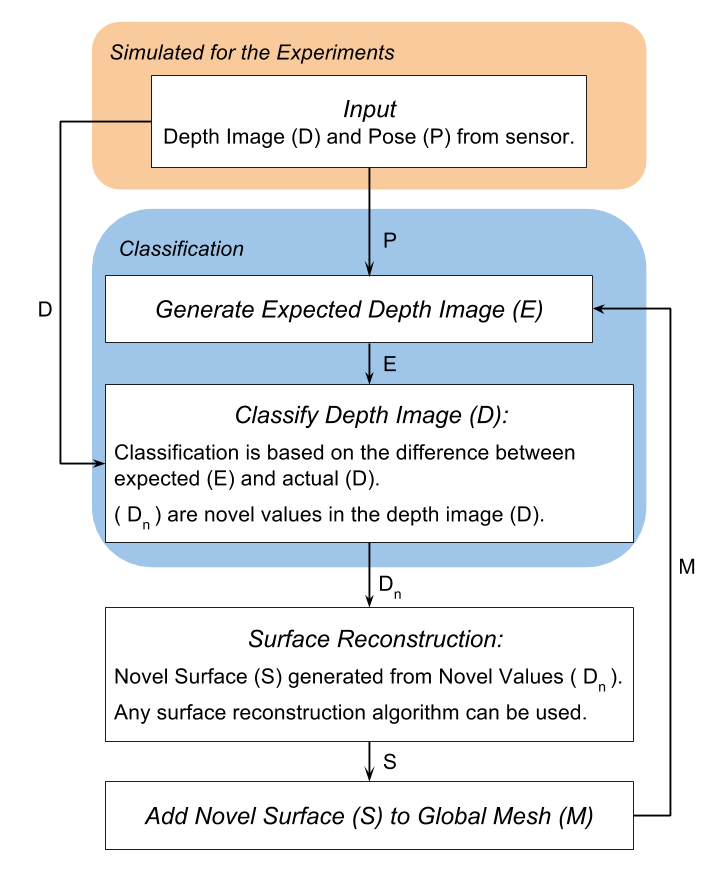
\includegraphics[width=.70\textwidth]{figures/diagram_system.png}
  \caption{MABDI system diagram}
  \label{fig:system}
\end{figure}

\begin{table}[h]
  \caption{Description of the main variables}
  \label{tab:var}
  \begin{center}
    \begin{tabular}{c|l}
    \cellcolor{white} {\bf Variable Name} & {\bf Description} \\ % adding \cellcolor{} here fixes the vertical line between the columns for some reason
    \rowcolor{LightGray}
    $D$ & Depth image from RGB-D sensor \\
    $P$ & Pose of the sensor \\
    \rowcolor{LightGray}
    $D_n$ & Parts of $D$ that are \emph{novel} \\
    $S$ & Novel surface generated from $D_n$ \\
    \rowcolor{LightGray}
    $M$ & Global mesh \\
    \end{tabular}
  \end{center}
\end{table}

The system diagram of Fig. \ref{fig:system} is a more detailed version of the
diagram seen in Fig. \ref{fig:pipeline_mabdi}. The ``Identify Novel Data''
component, shown in Fig. \ref{fig:pipeline_mabdi}, corresponds with the
Classification component, shown in blue. This Classification component is
MABDI's contribution to the state-of-art in mesh based mapping algorithms, and
is what gives MABDI the ability to make decisions about the incoming data. The
Classification component consists of two parts:
\begin{enumerate}
    \item \textit{Generate Expected Depth Image $E$} - Here we take the global
    mesh $M$, render it using computer graphics, and use the depth buffer of the
    render window to create a depth image $E$ of what we expect to see from our
    sensor. This method requires the current pose $P$ of the actual sensor
    (simulated for our experiments).
    \item \textit{Classify Depth Image $D$} - Here we classify the actual depth
    image $D$ (simulated for our experiments) by first taking the absolute
    difference between $E$ and $D$ and thresholding, as shown in the equation
    below. If the differences are small, those points are thrown away and if the
    differences are large, those points are kept as $D_n$. The idea behind this
    is, if the difference is large, the measurements are coming from a part of
    the environment that has not been seen before, i.e. novel. We found
    $threshold\mathsmaller{=}0.01$ worked well in our simulations. The
    implication of assuming all large differences signifies novel data is that
    this version of MABDI cannot handle object removal. It is worth noting that
    MABDI can be extended to handle object removal by using the sign of the
    difference between $E$ and $D$ instead of the absolute value.
    \begin{equation}
      D_n = \lvert D - E \rvert > threshold
      \label{eqn:d_e_diff}
    \end{equation}
\end{enumerate}

% Simulated for the Experiments
The system diagram in Fig. \ref{fig:system} also shows the Input and the Surface
Reconstruction components. The Input component has been simulated for our
experiments. More details of this simulation will be covered in Chapter
\ref{chapter:experimental_setup}. The Surface Reconstruction component of the
MABDI algorithm can be implemented with any viable surface reconstruction
method. Our implementation utilizes the structural information contained within
the depth image. We will discuss this in more detail in the next section.

\section{Implementation}

\subsection{Surface Reconstruction}
\label{subsection:surface_reconstruction}

The Surface Reconstruction component, as shown in Fig. \ref{fig:system}, is
responsible for creating a surface $S$ from the novel points $D_n$. The surface
$S$ is a mesh data structure that consists of a list of vertices and elements.
Vertices are points and elements define connections between vertices. Our method
outputs a triangle mesh, and so elements define the connection between three
vertices. $D_n$ is a subset of $D$ and is a list of pixel locations. For this
discussion, it will also be useful to define $D_k$ as the set of pixels in $D$
that are not pixels of $D_n$, shown in the equation below. $D_{known}$ is
labeled with ``\emph{known}'' because it represents data from the not novel or
``known'' parts of the environment. In the equation below ``$\setminus$'' is the
set difference operator.

\begin{equation}
D_{known} = D \setminus D_n
\end{equation}

Our surface reconstruction method first defines $S$ using all pixels from $D$.
We define the topology of the elements on the depth image. We can do this
because a depth image is not a set of unorganized points, but has inherent
structural information. This characteristic of the depth image allows us to
define a topology on the 2D depth image that is preserved when projected to 3D
coordinates. The topology we define can be visualized in Fig. \ref{fig:sr_t}.
Elements of the mesh are shown in light blue and pixels from $D$ are shown as
blue dots. Next we will identify elements to remove from $S$.

\begin{figure}[h]%[thpb]
\centering
  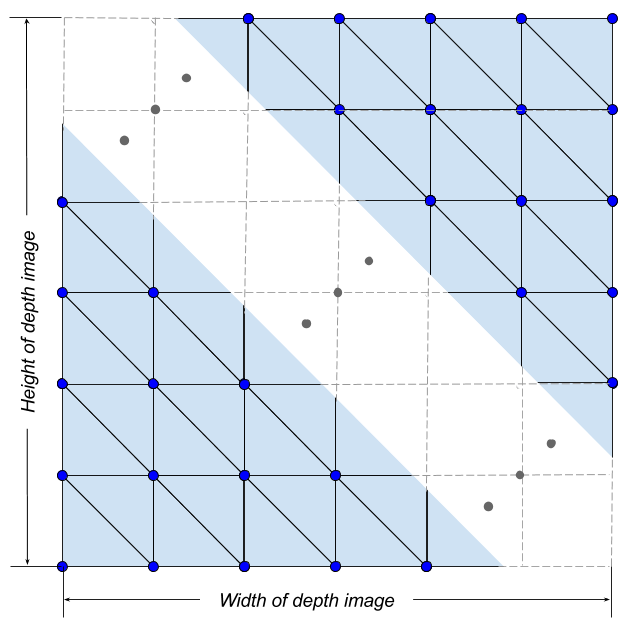
\includegraphics[width=.70\textwidth]{figures/diagram_sr_topology.png}
  \caption{Topology defined on the depth image (not all elements are shown)}
  \label{fig:sr_t}
\end{figure}

In order to remove elements defined by points that lie on completely different
surfaces, we use an imaging technique in the form of a convolution filter. A two
dimensional, differencing convolution filter is passed over $D$. This filter has
a magnified response at points where the difference between neighboring pixels
is large. Remembering pixel values signify depth, it is assumed pixels with
large differences between themselves and their neighbor lie on different
surfaces and therefore lie on the ``boundary'' of the real surface. A large
difference is defined by thresholding on the result of the convolution. We found
$threshold\mathsmaller{=}0.01$ worked well in our simulations. (The threshold
value is unitless because the depth image is defined by the z-component of the
view coordinates, which are normalized between 0 and 1.) Pixels identified
through this thresholding are marked as $D_{boundary}$ and are defined by the
equation below where $K$ signifies the kernel of the differencing convolution
filter.

\begin{gather}
  K = \begin{bmatrix} 2 & -1 \\ -1 & 0 \end{bmatrix} \\
  D_{boundary} = (D \ast K) > threshold
\end{gather}

Elements are removed from the $S$ if they touch pixels from the sets:
\begin{itemize}
  \item $D_{known}$ - Pixels from the known parts of the environment.
  \item $D_{boundary}$ - Pixels that lie on the boundary of the actual surface.
  \item $D_{invalid}$ -  Pixels that are invalid measurements. The RGB-D sensor
  naturally has pixels that are invalid, for example, those that are out of
  range.
\end{itemize}

Let us combine the sets defined above into one set $D_{throwaway}$:
\begin{equation}
  D_{throwaway} = D_{known} \cup D_{boundary} \cup D_{invalid}
  \label{eqn:throwaway}
\end{equation}

Our method removes elements that contain pixels from the set $D_{throwaway}$.
This can be seen in Fig. \ref{fig:sr_em}. Red dots signify pixels from
$D_{throwaway}$ and elements that contain these pixels are removed from $S$. In
the final step, all pixels are projected into 3D coordinates using the
transformation matrix of the sensor. These coordinates are the vertices of $S$.

\begin{figure}[h]%[thpb]
\centering
  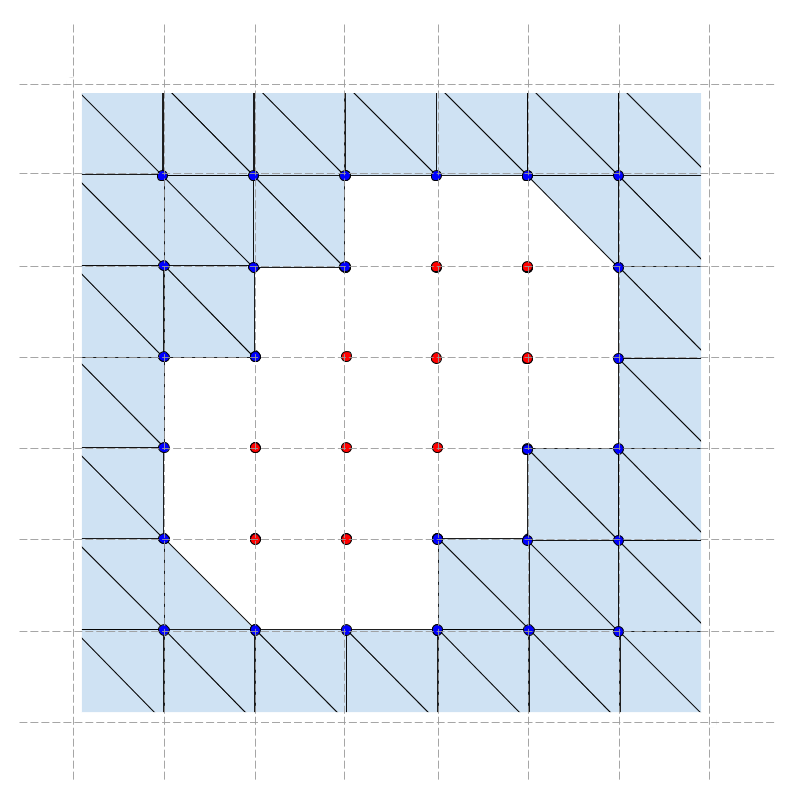
\includegraphics[width=.70\textwidth]{figures/diagram_sr_element_removal.png}
  \caption{Removal of elements}
  \label{fig:sr_em}
\end{figure}

Our surface reconstruction method was chosen for its ability to be implemented
simply and run quickly. One consequence of our method is that the resulting
surface $S$ can have a large number of elements. For example, if no points are
contained in the set $D_{throwaway}$ (this can happen on the first frame), $S$
will contain over 600,000 elements. We can see this by looking at Fig.
\ref{fig:sr_t}, assuming a depth image of size 640$\times$480, and considering
the equation below.

\begin{equation}
  612,162 = ((640-1)\times2)\times(480-1)
\end{equation}

Many surface reconstruction methods have been developed to create a surface more
intelligently than our surface reconstruction method, as discussed in Chapter
\ref{chapter:related_works}. For example, the advancing front method developed
by Marton et al. \cite{Marton2009} is capable of creating surfaces with fewer
elements than our method by utilizing a robust resampling method. A capability
of the MABDI algorithm is that the method developed by Marton et al. can be used
in place of our surface reconstruction method. This characteristic of MABDI is
advantageous because MABDI does not depend on the choice of surface
reconstruction method and the method can be chosen as the state-of-the-art
changes or to suit a particular application. Also, due to our implementation's
modular software design, the entire code base would not need to be changed in
order to accomplish this. We will discuss the software design in the next
section.

\subsection{Software Design}

From a software perspective, the major difficulty of implementing the MABDI
algorithm was found to be creating both the simulated depth image $D$ and the
expected depth image $E$. In addition, managing the complexity of the data
pipeline needed to run the algorithm and the simulation of the sensor proved to
be difficult. Thankfully, Kitware, which is a leading edge developer of
open-source software, created the Visualization Toolkit (VTK)
\cite{schroeder2004visualization, sitevtk}. At the time of this writing the VTK
Github repository has over 60,000 commits and is contributed to by supporters
such as Sandia National Labs \cite{sitesandia}.

VTK is suitable for the implementation of MABDI for many reasons. Perhaps
the most important is the concept of a vtkAlgorithm (often called a Filter).
This allows a programmer to create a custom and modular processing pipeline by
defining classes that inherit vtkAlgorithm and then defining the connections
between these classes. For example, you could have a pipeline that reads an
image from a source (component 1), performs edge detection (component 2), and
then renders the image (component 3).

Using the concept of VTK filters, the individual elements of MABDI can be
succinctly defined in individual classes. With that in mind, we can see in Fig.
\ref{fig:software} the layout used in our implementation of MABDI. vtkImageData
and vtkPolyData are VTK types used to represent an image and mesh respectively.
The elements shown in blue in Fig. \ref{fig:software} are the core components of
the MABDI algorithm and are implemented as custom VTK filters. Their source code
is included in Appendix \ref{appendix:mabdi_code}. Here we will discuss all
components in detail:

\begin{sloppypar}
\begin{itemize}
    \item  \textit{Source} - Classes with the prefix Source define the
    environment that is used for the simulation and provide a mesh in the form
    of a vtkPolyData.
    \item \textit{FilterDepthImage} - Render the incoming vtkPolyData in a
    window and output the depth buffer from the window as a vtkImageData. The
    output additionally has pose information of the sensor.
    \item \textit{FilterClassifier} - Implements the true innovation of MABDI,
    i.e., takes the difference between the two incoming depth images
    (vtkImageData) and outputs a new depth image where the data that is not
    novel is marked to be thrown away.
    \item \textit{FilterDepthImageToSurface} - Performs surface reconstruction
    on the novel points. For more detail see Section
    \ref{subsection:surface_reconstruction}. The surface is output as a
    vtkPolyData.
    \item \textit{FilterWorldMesh} - Here we simply append the incoming novel
    surface to a growing global mesh that is also output as a vtkPolyData.
\end{itemize}
\end{sloppypar}

\begin{figure}[b]%[thpb]
\centering
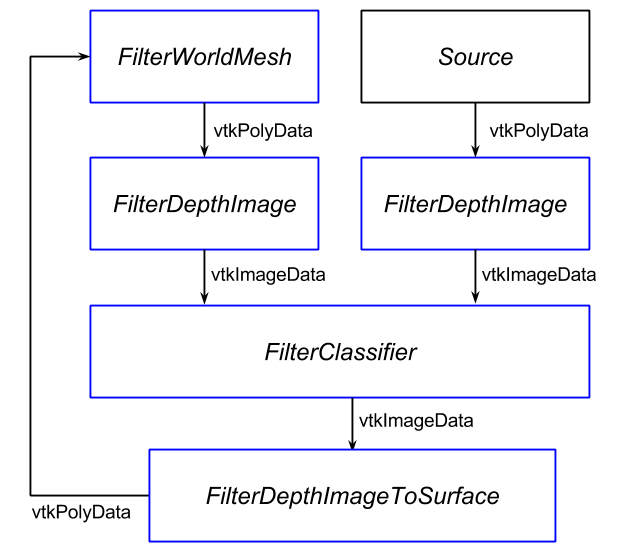
\includegraphics[width=.75\textwidth]{figures/diagram_software.png}
\caption{MABDI software diagram}
\label{fig:software}
\end{figure}

MABDI is implemented in Python and uses VTK. Our implementation is distributed
under the BSD license and is available on Github at the address below:

$$
https://github.com/lucasplus/MABDI
$$

At the time of this writing, it consists of over 1,400 lines. The code that
implements the MABDI algorithm itself is around 750 lines.
